\chapter{CHVote Protocol}
Our project is based on the CHVote protocol specifications. We would like to point out, that this protocol and the followign ideas do not originate from us! The concept and specifications have been created by Rolf Haenni, Philipp Locher and Reto E. Koenig of the Institute for Security in the Information Society (RISIS) of the Bern University of Applied Sciences. For this project, we have implemented the protocol according to their specification. In this section we summarize the most important aspects of the protocol and establish the terminology for better understanding this document and our application

\section{Actors}
A \textbf{voter} is a person who is eligible to vote in his respective state. Every voter is assigned a \textbf{counting circle} which typically corresponds to the voters municipal and is required for statistical purposes. For authentication purposes, every voter must possess a voting card that has been sent to him prior to an election event that contains codes used to identify the voter during the vote casting process.

The \textbf{Election Administrator}, typically a person of the government, is responsible for setting up the election event by providing the required information such as the candidates or the voters and initiates the generation of the cryptographic electorate data. He is also responsible for tallying the election and publishing the final results.

The \textbf{election authorities} can be seen as some kind of independent election observers. In a CHVote election event there are always multiple election authorities in order to avoid having to trust a single authority. The authorities are involved in almost every step of the protocol, starting from the generation of their shares of the electorate data, checking and responding to new ballots, as well as in the mixing (a measure to ensure anonymity) and decryption phases. The public key that is used for encrypting the ballots has been jointly generated by all election authorities. Therefore in order to decrypt the ballots, all authorities must work together and provide their share of the private key. 

The measure of multiple authorities participating in the whole e-voting process establishes a \textbf{distribution of trust} and ensures security of the whole election process as long as at least one election authority can be trusted.

The \textbf{Bulletin Board} acts as a central board over which most communication is done and where all the public data is stored. By publishing all data that is not secret onto a public board, including the list of encrypted ballots, and functionality to verify the correctness of these data, the protocol is making a big step towards the demanded transparency and the universal verification.

The \textbf{Printing Authority} is responsible for printing the voting cards for all voters. Since the printing authority needs to be in possession of all the secret voting codes, it is a very sensitive point in the protocol. The printed voting cards are handled over to a trusted mailing service for delivery.

\section{Pre-Election \& Voting Cards}
Before the actual election phase, the vote administrator sets up the election event by entering all required parameters, including the voters, the elections with their corresponding candidates and the number of candidates a voter can select in every election. All election authorities jointly generate the cryptographic data for the whole electorate from which the voting card information is derived. The printing authority combines the information from all election authorities, prints the voting cards and delivers them to the voters by a trusted mailing service. 

A voting card contains several codes, namely:

\begin{itemize}
	\item a voting code
	\item a confirmation code
	\item a finalization code
	\item one verification code for every candidate
\end{itemize}

The \textbf{voting and confirmation codes} are authentication codes and are used to authenticate the voter twice during the vote casting process; the first time with the voting code when he casts his vote, and a second time for confirming his vote. A second authentication code is required because otherwise an attacker who infected a voters computer with malware could just confirm a vote on behalf of the voter after he manipulated the candidate selection and could therefore skip the whole verification process.

\section{Vote casting with oblivious transfers}
As mentioned earlier, one of the big challenges of an evoting-protocol is how it deals with the insecure platform problem: A voting platform that is infected with malware poses the risk that an attacker can manipulate the candidate selection on the vote-casting page after the voter has entered his voting code. 

The CHVote specification suggests a "`Cast-as-intended verification"'-step to allow voters to detect this kind of manipulation: When a voter enters his voting code and the indices of his favored candidates, the voting client forms a \textbf{ballot} containing the voters selection encrypted with the authorities public key, his public voting credential derived from the voting code, and a \textbf{non-interactive zero knowledge proof} which proofs that the voter has formed the ballot according to the protocol and that he has been in knowledge of his voting code, without revealing any information about the voting code.

Every election authority has to check the voters public voting credential, the validity of the ballot proof and that the voter hasn't already cast a vote. The encrypted selection also serves as a query for an oblivious transfer. A \textbf{k-out-of-n oblivious transfer} allows a client to query a server for $k$ messages, without the server knowing what messages the client requested, and without the client learning anything about the other $n-k$ messages. Adapted to the CHVote protocol: The voting client queries the authorities for the corresponding verification codes of the selected candidates, without the authorities learning which candidates the voter has selected, and without revealing any information about the other candidates. 

The voter then checks if the returned verification codes match the codes of the candidates he has chosen on the printed voting card. If the selection was somehow manipulated by malware, the returned verification codes would not match the printed ones and the voter would have to abort the vote casting process. This way the integrity of the vote casting process can be guaranteed even in the presence of malware. In such a case, privacy on the other hand cannot be protected since the malware will learn the plaintext of the voters selection.

Another feature the protocol supports, is that an election event can consist of $t$ multiple parallel elections. In such cases, the voter has to submit a single ballot, which contains his candidate selection for all parallel elections. This raises the question, how the system can verify that a voter has chosen exactly the correct number of candidate in each election, and not for example one less in the first, and one additional candidate in the second election.

The specification suggests the following trick: Assuming an election consists of two parallel elections ($t=2$) with 3 candidates each ($n_1 = 3, n_2 = 3$), of which a voter can select one candidate in each election ($k_1 = k_2 =1$). The verification codes are derived from $n = \sum_{j=1}^{t} n_j$ random points on $t$ polynomials (one for every election event $j$) of degree $k_j - 1$, that each election authority has chosen randomly prior to the election. By learning exactly $k = \sum_{n=1}^{t} k_j$ points on these polynomials, the voting client is able to reproduce these polynomials and therefore is able to calculate a particular point with $x=0$ on these polynomials. The corresponding $y$ values are incorporated into the second credential from which the confirmation code is derived. As a result, only if a voter has been able to reconstruct these polynomials with the returned points by submitting a valid candidate selection, he will be able to confirm the vote that he casted.

\section{Anonymity with a Рe-Еncryption Mix-Net}

As mentioned earliert, both the election authorities as well as the bulletin board keep track of all the casted ballots, which contains the voters candidate selection encrypted under the public key that has been jointly generated by all election authorities. Up to this point, the ballots are still linked to the voters, since the voter identifier is required for the confirmation process and to avoid that a voter can cast multiple ballots. If the ballots were decrypted now, this would conflict with the anonymity and the privacy of the voters.

As the first step of the post-election phase, the first election authority extracts the encrypted candidate selections from the ballots. In order to anonymize this list of encryptions, the protocol suggests a "`mixing-process"', in which every authority performs a cryptographic shuffle with a random permutation. Additionally, all the encryptions are re-encrypted such that they receive a new ciphertext. This re-encryption is done by using the multiplicative homomorphic property of the ElGamal encryption scheme that is used for encrypting the ballots. A \textbf{multiplicative homomorphic encryption} scheme allows to perform multiplications on the ciphertext such that:

\begin{equation*}Enc(a) \cdot Enc(b) = Enc(a \cdot b)\end{equation*}

The specification suggests multiplying the encrypted selection with the encryption of the neutral element $1$ since this yields a new ciphertext for the exact same plaintext.

\begin{equation*}Enc(a) \cdot Enc(1) = Enc(a)\end{equation*}

\begin{center}
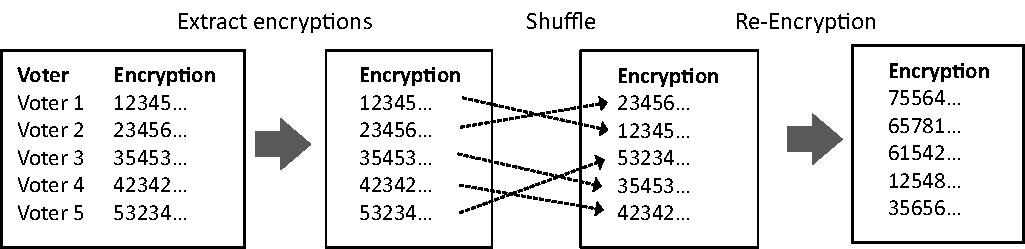
\includegraphics[scale=0.95]{assets/mixing.pdf}
\captionof{figure}{During the mixing phase, the encryptions are extracted from the list of ballots and then shuffled with a random permutation and re-encrypted by all election authorities. This measure ensures the anonymity of the votes. }\label{During the mixing}%
\end{center}

While the extraction only needs to done by the first election authority, every election authority is sequentially performing the shuffle and re-encryption on the mixed list of the previous election authority.

To prevent election authorities from cheating and not performing the mixing as specified, a proof (according to Wikström’s shuffle proof) is calculated which will be verified by all election authorities before decryption. If one of these \textbf{shuffle-proofs} fails, the election process can not proceed.
